\documentclass[10pt,a4paper]{article}

\usepackage[margin=1in]{geometry}
\usepackage{graphicx}
\usepackage{longtable}
\usepackage[dutch]{babel}
\usepackage{url}
\usepackage{minted}
\usepackage{caption}
\usepackage{subcaption}
\usepackage{amsmath, amsthm, amssymb,amsfonts}

\usepackage[section]{placeins}

\usepackage{algorithm}
\usepackage{algpseudocode}
\newcommand*\Let[2]{\State #1 $\gets$ #2}

\usepackage{color}

\usepackage{wrapfig}

\usepackage{rotating}
\usepackage{float}

\usepackage{gensymb}

\usepackage{xypic}
\usepackage[all,color]{xy}
\xyoption{all}

\usepackage{epstopdf}
\epstopdfDeclareGraphicsRule{.tif}{png}{.png}{convert #1 \OutputFile}
\AppendGraphicsExtensions{.tif}

\usepackage{fancyhdr}
\pagestyle{fancy}
\fancyhead{}
\fancyfoot{}
\renewcommand{\headrulewidth}{0mm}
\rfoot{\thepage}    
\cfoot{}
\lfoot{CV finaal project: Snijtand Segmentatie - Christophe Van Ginneken (s0084580)}

\definecolor{bg}{rgb}{0.95,0.95,0.95}

\geometry{a4paper}

% http://tex.stackexchange.com/questions/299/how-to-get-long-texttt-sections-to-break
\newcommand*\justify{%
  \fontdimen2\font=0.4em% interword space
  \fontdimen3\font=0.2em% interword stretch
  \fontdimen4\font=0.1em% interword shrink
  \fontdimen7\font=0.1em% extra space
  \hyphenchar\font=`\-% allowing hyphenation
}

% http://en.wikibooks.org/wiki/LaTeX/Customizing_LaTeX
\newcommand{\ttt}[1]{{\tt \justify{#1}}}

\author{Christophe Van Ginneken (s0084580) \\
	\url{Christophe.VanGinneken@student.kuleuven.be} }
\title{CV finaal project: Snijtand Segmentatie}

\begin{document}

\maketitle

\vspace{-1cm}
\section*{Introductie}

In dit project wordt het segmenteren van snijtanden op basis van radiografie\"en bestudeerd. We vertrekken hierbij van bestaande literatuur, uit de welke een strategie gekozen en ge\"implementeerd wordt. De resultaten van deze implementatie worden besproken in het kader van de cursus.

Dit rapport volgt dezelfde structuur: eerst worden enkele van de geconsulteerde rapporten kort toegelicht, waaronder ook de geselecteerde strategie. De implementatie wordt besproken en de uitdagingen die er in vervat zaten worden geanalyseerd. Tot slot worden de resultaten besproken en worden conclusies getrokken.

De belangrijkste resultaten en code voorbeelden zijn opgenomen in dit rapport, in de tekst of in appendices. Alle broncode die gebruikt werd bij de realisatie van de gekozen strategie, is ook online beschikbaar via \url{http://github.com/MyKULCourses/cv} in de folder \ttt{final}.

\section*{Literatuur studie}

Enkele van de aangeboden, alsook andere opgezochte artikels werden verwerkt. In deze sectie worden ze kort samengevat.

\subsection*{Challenges of Developing an Automated Dental Identification System}

In \cite{abdel2003challenges} wordt een strategie voorgesteld die uit twee stappen bestaat: eerst wordt een tweeledige methode op basis van drempelwaarden toegepast waarna door middel van integrale projectie de individuele tanden gesegmenteerd worden. Het bepalen van de effectieve contour wordt nauwelijks beschreven en wordt opgenomen in het gedeelte over het vergelijken van de ante- en post-mortem informatie.

Deze methode bestaat uit de toepassing van een iteratieve en een adaptieve drempelwaarde. De iteratieve drempelwaarde wordt ge\"implementeerd aan de hand van een \emph{Canny} rand detectie. De adaptieve drempelwaarde wordt gerealiseerd door middel van morfologische dilatatie, toegepast op het beeld van binaire randen. Op deze manier worden de pixels rond de randen gevonden. Van de overeenkomstige pixels wordt een gemiddelde grijs-waarde bepaald, die als initi\"ele drempelwaarde gebruikt wordt. Deze waarde zorgt voor een opdeling in tand- en achtergrondgebieden. Via een iteratief proces wordt deze waarde bijgesteld tot ze convergeert.

Door het toepassen van een adaptieve drempelwaarde, wordt vervolgens een binaire opdeling gemaakt tussen tanden en achtergrond. Deze drempelwaarde wordt toegepast op het originele beeld dat eerst gemaskeerd wordt met het iteratief bekomen masker.

Dit binaire beeld vormt vervolgens de basis voor het segmenteren van de individuele tanden. Hier wordt eerst gezocht naar een horizontale splitsing tussen onder- en bovenkaak. Hierbij wordt een minimale som van horizontale intensiteiten gezocht. Aangezien achtergrondgebieden zwart zijn, zal een overwegend zwarte scheidingslijn een zeer lage, gesommeerde intensiteit kennen en duiden op een splitsing. Omdat deze horizontale lijn niet altijd mooi horizontaal zal zijn, wordt een rotatie van deze lijn tussen -20\degree en +20\degree in rekening genomen. Aangezien dit niet altijd mogelijk is, wordt voorgesteld om dit te doen voor verticale deelgebieden.

Vertrekkende van deze horizontale splitsing worden de tanden ge\"isoleerd. Hierbij wordt een gelijkaardige methode toegepast en wordt vanaf de horizontale splitsing gezocht naar rechten die loodrecht staan op de splitsing, met opnieuw in acht nemen van een hoek tussen -20\degree en +20\degree, waarbij de som van de intensiteiten opnieuw minimaal is.

Het vervolg van dit artikel focust hoofdzakelijk nog op het opslaan en het terugvinden door vergelijken van de informatie over de individuele tanden.

\subsection*{Active Contour Based Segmentation of Low-Contrast Medical Images}

In \cite{abdel2003challenges} wordt verwezen naar \cite{piotrowski2000active}, een artikel dat in het algemeen het probleem van contour detectie in laag-contrast medische beeldvorming aanpakt. Het artikel beschrijft enkele aspecten: eerst wordt de normalisatie van de originele beelden voorgesteld op basis van het zgn. \emph{contrast stretching}. Vervolgens wordt een initi\"ele contour detectie gedaan door middel van Hough transformaties. Aan de hand van een energie functie wordt deze initi\"ele vorm vervolgens verbeterd tot het finale resultaat.

Het dient opgemerkt te worden dat de segmentatie door toepassing van achtereenvolgens een Sobel filter, een drempelwaarde en Hough transformaties wel een beperking oplegt dat er bv.\ slechts \'e\'en tand in het beeld aanwezig mag zijn.

Het minimaliseren van de contour energie wordt gedaan door middel van \emph{simulated annealing} en kent vier fasen:

\begin{enumerate}
\item In de \emph{browsing} fase kan de vorm zeer vrij bewegen, met zeer weinig beperkingen.
\item Tijdens \emph{setting the macro-state} fase blijven contouren meer gelokaliseerd.
\item Daarna zal de contour beginnen oscilleren rond de rand van het object.
\item In de laatste fase, \emph{freezing in de local minimum} wordt door de lage \emph{temperatuur} het simulated annealing proces beperkte tot een \emph{downhill search}.
\end{enumerate}

\subsection*{Tooth Contour Extraction for Matching Dental Radiographs}

De verwijzing naar actieve contouren in algemeen, laag-contrast medische beelden leidde naar \cite{chen2004tooth}, een zeer beknopt artikel waarin een strategie wordt voorgesteld op basis van actieve contour modellen of zgn. \emph{snakes} om specifiek contouren van tanden te bekomen. Omdat hierbij het probleem kan rijzen van interferentie van naburige tanden, stellen ze tevens een nieuwe dynamische energie term voor. Hierbij wordt gebruik gemaakt van gradi\"ent richtingen. In het geval van tanden is dit mogelijk omdat bij een gerichte \emph{snake} de tand steeds aan dezelfde kant zal liggen.

Dit artikel verwijst naar \cite{jain2004matching}, een artikel van dezelfde auteurs, en vermeldt dat de daarin voorgestelde strategie op basis van een intensiteiten distributie model, snel zal falen indien de contouren wazig zijn of er zich overlappingen voordoen. Anderzijds wordt de structurele aanpak voor de segmentatie van tanden wel weerhouden bij de initialisatie fase.

Voor de detectie van de contouren wordt eerst gezocht naar de scheidingslijn tussen tandvlees en achtergrond. Hierdoor worden de kroon en de wortel gescheiden. Vervolgens wordt de methode van \cite{jain2004matching} toegepast om een initi\"ele \emph{snake} te bekomen. Door een convergentie naar de gradi\"ent  wordt dit initi\"ele resultaat verbeterd tot het finale resultaat.

\subsection*{Dental X-ray Image Segmentation}

\cite{said2004dental} is een artikel dat duidelijk volgt op \cite{abdel2003challenges} en uitgebreider ingaat op het concept \emph{contrast stretching}, zoals ook beschreven in \cite{piotrowski2000active}.

Initieel kent het artikel een zeer lange beschrijvende inleiding, waarin de context van het segmenteren van tanden uiteen gezet wordt. Vervolgens wordt een methodologie voorgesteld. Een eerste stap bestaat uit het verbeteren van de beelden door middel van \emph{contrast stretching}. Naast de theoretische onderbouw voor \emph{contrast stretching} wordt niet verder ingegaan op de implementatie ervan. Wel wordt aangegeven dat tijdens de voorbereiding van de beelden een \emph{Top-Hat} filter nodig is om het onderscheid tussen tanden en botten mogelijk te maken.

Vervolgens wordt opgemerkt dat voor segmentatie twee strategie\"en kunnen gevolgd worden: enerzijds de extractie op basis van regionale kenmerken en anderzijds op basis van modellen. Deze laatste strategie is complexer, maar dikwijls meer succesvol.

De methodologie gaat tot slot verder met een summiere beschrijving van de segmentatie door middel van 2D wavelets en concludeert dat deze aanpak veruit de beste is, in vergelijking met andere aanpakken.

\subsection*{Matching of dental X-ray images for human identification}

In \cite{jain2004matching} wordt ook een tweeledige methodologie voorgesteld: eerst een segmentatie van de individuele tanden en vervolgens een extractie van de effectieve contouren. De auteurs van het artikel geven zelf aan dat hun aanpak waarschijnlijk niet geschikt is voor een volledig automatische verwerking van grote sets en dat fouten in problematische situaties manueel dienen gecorrigeerd te worden. Ook adviseren ze om waar mogelijk manueel een initi\"ele aanduiding te geven van verwachte locaties, zoals voor de splitsing tussen de onder- en bovenkaak. Desalniettemin beschrijven ze een strategie die volledig geautomatiseerd kan worden.

De scheiding van onder- en bovenkaak volgt het principe dat voorgesteld werd in \cite{abdel2003challenges}, en zoekt splitsingen aan de hand van histogrammen van de horizontale en verticale intensiteiten, echter zonder de bijkomende variatie van de hellingsgraad van -20\degree tot +20\degree. Ook wordt het principe van de verticale banden gehanteerd. De resulterende hoogtes van de splitsingen worden vervolgens als basis genomen om een interpolerende \emph{spline} te bepalen.  Het zoeken van splitsingen tussen individuele tanden wordt vervolgens gedaan volgens rechten die loodrecht staan op deze \emph{spline}. Op basis van deze splitsingen kunnen ROI's bepaald worden die telkens (hoofdzakelijk) \'e\'en tand bedekken. 

Een ROI wordt vervolgens opgedeeld in een kroon en een wortel door middel van het identificeren van een kroon centrum halverwege de breedte en op $\frac{1}{3}$ van de top van de ROI. Via een distributiemodel van intensiteiten wordt vervolgens via een tracering van een halve cirkel de contour van de kroon bepaald. In een volgende fase wordt de wortel verder getraceerd. Hierbij wordt gewerkt met een contrast verschil omdat deze regio veel waziger is wegens de combinatie van tand en kaakbeen dat gelijkaardige intensiteiten oplevert.

De overige helft van het artikel gaat dieper in op het opslaan en vergelijken van ge\"identificeerde tanden.

\section*{Implementatie strategie}

Voor de implementatie van dit project werd uitgegaan van \cite{jain2004matching} als basis algoritme met toepassing van  \emph{contrast stretching} zoals aangegeven in \cite{piotrowski2000active} en verder gedetailleerd in \cite{said2004dental}.

Omdat dit artikel veel geciteerd werd in de andere geconsulteerde werken en omdat het in grote lijnen een andere aanpak beschrijft dan deze die tijdens de lessen van de cursus voorgesteld werd, leek het een interessante opportuniteit om na te gaan hoe deze methodologie effectief kan presteren op basis van een implementatie binnen een kort tijdsbestek.

Vooral de aanpak om een volledige radiografie van een gebit te segmenteren in individuele ROI's wordt meermaals geciteerd. Ook worden enkele complexiteiten uit andere artikels anders opgelost. Zo wordt bv.\ gebruik gemaakt van een \emph{spline} functie om de splitsing tussen onder- en bovenkaak te beschrijven. Dit in tegenstelling tot de variabele hoek in \cite{abdel2003challenges}.

Zoals aangegeven in \cite{chen2004tooth} verwachten we inderdaad dat er mogelijke problemen zullen optreden bij beelden waarbij de contouren wazig zijn of waar er zich overlappingen voordoen. Dit laatste is niet ongewoon bij vervormingen en komt in een radiografie tot uiting door overlappingen van de beelden van de individuele tanden.

\section*{Implementatie}

In dit deel bespreken we de implementatie van de gekozen strategie. Hierbij bekijken we eerst de structuur van het project met de verdeling van verantwoordelijkheden over gekozen technologie\"en en de structurele opdeling in scripts.

Vervolgens doorlopen we de implementatie zelf. Hierbij bespreken we de aanpak zoals deze voorgesteld werd in de literatuur en geven we aan welke aannames werden gedaan of waar aanpassingen werden doorgevoerd om bepaalde problemen te verhelpen.

\subsection*{Structuur}

De resulterende code is hoofdzakelijk geschreven in Python, maakt gebruik van de OpenCV, NumPy en SciPy bibliotheken. Daarnaast werd geopteerd om de co\"ordinatie en aansturing van deze code te doen vanuit een doel-geori\"enteerde \ttt{Makefile}. Hierdoor is er een sterke scheiding tussen configuratie en aansturing enerzijds en algoritme en uitvoering anderzijds. Zaken als bepalen welke bestanden geladen moeten worden of welke logica dient uitgevoerd te worden is op deze manier gecentraliseerd en niet verspreid over de verschillende Python bestanden.

Voor elke fase of handeling die uitgevoerd wordt, is een apart Python script voorzien. Deze zijn opgezet als modules, maar kunnen ook op zich uitgevoerd worden. In dit laatste geval zal het script zijn functionaliteit uitvoeren en het resultaat interactief laten zien op het scherm. Deze werking wordt geactiveerd indien er geen uitvoerbestand wordt meegegeven aan de oproep.

Indien dit laatste wel wordt gedaan, is dit de naam van een \ttt{Matlab} bestand met extensie \ttt{.mat}. In plaats van de resultaten te visualiseren, worden deze nu opgeslagen in dit bestand. Deze bestanden worden tevens doorgegeven aan de volgende fase, waardoor er voor elke fase een onafhankelijke set van data- en uitvoer bestanden ontstaan. Het \ttt{Matlab} formaat werd gekozen omwille van interoperabiliteit. Zo zijn de scripts om grafieken, zoals histogrammen, te visualiseren gerealiseerd als \ttt{Matlab} scripts. Hierdoor zijn deze grafieken in dit verslag visueel conform aan geldende standaarden en kon ervaring op dit vlak hergebruikt worden.

Tot slot zijn er naast de interactieve manier om de resultaten te bekijken, ook overeenkomstige Python scripts gemaakt die de visualisatie realiseren naar een bestand.

De hele structuur is visueel weergegeven in figuur \ref{fig:setup}: van boven naar onder is de implementatiestrategie stap voor stap weergegeven in de vorm van rechthoeken met de naam van het overeenkomstige Python of Octave\footnote{Octave is een Open Source implementatie van de Matlab functionaliteit. Voor meer info zie \url{http://www.gnu.org/software/octave/}} script. Verticale pijlen duiden de logische opeenvolging aan en geven tevens aan welke bestanden uit een vorige fase gebruikt worden om verder te gaan. Horizontale pijlen geven de mogelijkheden tot visualisatie.

\begin{figure}
\centering
\[ \entrymodifiers={+++[F-]}
\SelectTips{cm}{}
\xymatrix {
	*{origineel} 											
		\ar[d]_{\tt 01.tif} \\
	\parbox{5.75cm}{\centering crop\_image.py} 
		\ar[d]_{\tt 01\_crp.tif} \\
	\parbox{5.75cm}{\centering create\_histogram.py} 
		\ar[d]_{\tt 01\_crp.tif}^{\tt 01\_crp\_histogram.mat}
		\ar[rr]^{\tt 01\_crp\_histogram.mat} &*{\hspace{2.5cm}} & \parbox{4cm}{\centering plot\_hist.m} \\
	\parbox{5.75cm}{\centering determine\_enhancement\_parameters.py} 
		\ar[d]^{\tt 01\_crp\_enh.mat} 
		\ar[rr]^{\tt 01\_crp\_enh.mat} &*{\hspace{2.5cm}} & \parbox{4cm}{\centering plot\_sigmoid.m} \\
	\parbox{5.75cm}{\centering create\_enhanced\_image.py}
		\ar[d]	_{\tt 01\_crp\_enh.tif}	 &*{\hspace{2.5cm}} & \parbox{4cm}{\centering plot\_jaw\_hists.m} \\
	*+++[F=]{\parbox{5.75cm}{\centering jaw\_split.py}}
		\ar[d]_{\tt 01\_crp\_enh.tif}^{\tt 01\_crp\_enh\_jaw\_split.mat}
		\ar[rru]^{\tt 01\_crp\_enh\_jaw\_split.mat}
		\ar[rr]^{\tt 01\_crp\_enh\_jaw\_split.mat}_{\tt 01\_crp\_enh.tif} &*{\hspace{2.5cm}} & \parbox{4cm}{\centering visualize\_jaw\_split.py} \\
	*+++[F=]{\parbox{5.75cm}{\centering teeth\_isolation.py}}
		\ar[d]	^{\tt 01\_crp\_enh\_teeth\_iso.mat}
		\ar[rr]^{\tt 01\_crp\_enh\_teeth\_iso.mat}_{\tt 01\_crp\_enh\_jaw\_split.mat} &*{\hspace{2.5cm}} & \parbox{4cm}{\centering visualize\_teeth\_isolation.py} \\
	*+++[F=]{\parbox{5.75cm}{\centering roi.py}}					
		\ar[d]	_{\tt 01\_crp\_enh.tif}^{\tt 01\_crp\_enh\_roi.mat}
		\ar[rr]^{\tt 01\_crp\_enh\_roi.mat}_{\tt 01\_crp\_enh\_teeth\_iso.mat} &*{\hspace{2.5cm}} & \parbox{4cm}{\centering visualize\_roi.py} \\
	*+++[F=]{\parbox{5.75cm}{\centering contours.py}}
		\ar[rr]^{\tt 01\_crp\_enh\_contours.mat}_{\tt 01\_crp\_enh\_roi.mat}
		\ar[d]^{\tt 01\_crp\_enh\_contours.mat}_{\tt 01\_crp\_enh\_roi.mat} &*{\hspace{2.5cm}} &  \parbox{4cm}{\centering visualize\_contours.py} \\
	\parbox{5.75cm}{\centering mask.py}
		\ar[rr]^{\tt 01\_crp\_enh\_masks.mat}_{\tt 01\_crp\_enh\_roi.mat} 
		\ar[d]^{\tt 01\_crp\_enh\_masks.mat}_{\tt 01\_crp\_enh\_roi.mat} &*{\hspace{2cm}} &  \parbox{4cm}{\centering visualize\_masks.py} \\
	\parbox{5.75cm}{\centering compare\_mask.py}	
}
\]
\caption{Overzicht structuur en werking}
\label{fig:setup}
\end{figure}

Het originele beeld wordt eerst voorbereid. Hierbij wordt het zeer algemeen bijgesneden (\ttt{crop\_image.py}) tot een beeld dat hoofdzakelijk de tanden bevat. Vervolgens wordt van dit beeld een histogram van de intensiteiten gemaakt (\ttt{create\_histogram.py}). Aan de hand van dit histogram wordt het beeld vervolgens verbeterd: eerst worden de parameters bepaald van de normalisatie functie (\ttt{determine\_enhancement \_parameters.py}) en vervolgens wordt het beeld effectief verbeterd (\ttt{create\_enhanced\_image.py}). Dit zijn algemene acties die het beeld voorbereiden voor het effectieve algoritme.

Dit algoritme bestaat uit vier grote fasen. Deze zijn in figuur \ref{fig:setup} weergegeven met dubbele omkaderende lijnen. Eerst wordt een splitsing gemaakt tussen de boven- en onderkaak (\ttt{jaw\_split.py}). Dan worden voor elk van deze kaken, splitsingen gezocht tussen de vier middelste tanden, waardoor deze ge\"isoleerd worden (\ttt{teeth\_isolation.py}). Op basis van deze splitsingen worden dan rechthoekige afbakeningen van de interessante regio gemaakt, de zgn. \emph{Region Of Interest} of \emph{ROI} (\ttt{roi.py}). Tot slot wordt binnen deze ROI's gezocht naar de contour van de tand (\ttt{contours.py}).

De contouren die bekomen worden zijn soms redelijk ruw ten gevolgen van ``fouten''. In de nabewerking worden deze contouren verzacht om zo definitieve contouren van de maskers te bekomen (\ttt{mask.py}). Tot slot worden nog visuele vergelijking gemaakt van de gekende maskers t.o.v.\ de zelf bepaalde maskers (\ttt{compare\_mask.py})

\subsection*{Voorbereiding}

Vooralleer de segmentatie en contour-afbakening kan gebeuren, is het aangewezen om het originele beeld voor te bereiden. De originele beelden zijn zeer ruim in functie van de scope van de opdracht. De opdracht focust op de acht snijtanden, daar waar de originele beelden de volledige kaken beslaan. Daarom werd besloten om als eerste stap een zeer ruwe ROI te bepalen, een zgn. macro-ROI.

Vervolgens dient ook het contrast verbeterd te worden. Hiervoor werd de techniek \emph{contrast stretching}, waar ook in  \cite{piotrowski2000active} en \cite{said2004dental} naar verwezen werd, gehanteerd.

\subsubsection*{Bepalen macro-ROI}

De originele beelden laten toe om de sterke structurele gelijkenissen uit te buiten en het volledige beeld te herleiden tot een kleiner beeld waar zich alleen de zone op bevindt die belangrijk is in dit project. Zonder te zoeken naar optimale maten, werd een ruwe bijsnijding ge\"implementeerd die het beeld herleidde tot een centrale regio van 700 pixels breed en 850 pixels hoog\footnote{De originele beelden zijn 3023 breed en 1597 hoog.}.

Zoals blijkt uit het overzicht van de voorbereide originele beelden in appendix \ref{appendix:prepared-originals}, kan deze bijsnijding is veel gevallen nog verbeterd worden. Er is echter geopteerd om deze begeleide operaties zo algemeen mogelijk uit te voeren om zo min mogelijke manuele interferentie te noodzaken. Hierdoor zijn de voorbereidingen redelijk ruw, maar zo weerspiegelen hopelijk de resultaten de kwaliteiten van de strategie in een geautomatiseerde omgeving waar zo min mogelijk interventie nodig is.

We kunnen nu reeds opmerken dat een aantal van de originele beelden problematische eigenschappen vertonen zoals schaduwen, corrigerende beugels en blokjes. Daarnaast zijn er ook een aantal beelden met sterk vervormde tand-formaties.

\subsubsection*{Verbeteren van het contrast}

Radiografie-beelden zijn gekenmerkt door een veelheid aan grijstinten en wazige overgangen. Omdat we op basis van histogrammen van intensiteiten splitsingen willen gaan bepalen, is het belangrijk dat er een duidelijk onderscheid is tussen donkere en lichte zones. Om deze reden is het belangrijk om te zorgen voor een accentuering van het contrast, waarbij donkere zones expliciet donkerder gemaakt worden en lichtere zones lichter. Een techniek die dit doet is het zogenaamde \emph{contrast stretching}.

Zoals de naam doet vermoeden trachten we bij \emph{contrast stretching} het contrast dat er is, zo uit te rekken, dat het nadrukkelijker aanwezig is. Om dit te doen, werken we met een histogram van de intensiteiten van de grijs-waarden en defini\"eren we een transformatie van deze intensiteiten. Figuur \ref{fig:contrast-stretching-histograms} toont een histogram v\'o\'or en na \emph{contrast stretching}. Het is duidelijk dat de intensiteiten nu als het ware uitgerokken zijn over het volledige spectrum en dat de stretching vooral in de middelste zone gebeurd is. Merk op dat door het uitrekken er ook gaten ontstaan.

\begin{figure}
\centering
\begin{subfigure}{.49\textwidth}
  \centering
  \includegraphics[width=.9\linewidth]{../01_crp_hist.eps}
  \caption{Origineel}
  \label{fig:original-histogram}
\end{subfigure}
\begin{subfigure}{.49\textwidth}
  \centering
  \includegraphics[width=.9\linewidth]{../01_crp_enh_hist.eps}
  \caption{Na verbetering}
  \label{fig:enhanced-histogram}
\end{subfigure}
\label{fig:contrast-stretching-histograms}
\caption{Histogrammen voor en na contrast stretching van \ttt{01\_crp.tif}}
\end{figure}

Als transformerende functie werd een \emph{sigmoid} functie gebruikt. Vergelijking \ref{eq:sigmoid-standard} toont de algemene vorm.

\begin{equation} \label{eq:sigmoid-standard}
(newMax - newMin) \frac{1}{1+e^{-\frac{I - \beta}{\alpha}}} + newMin
\end{equation}

In dit geval beelden we het intensiteiten interval $[0..255]$ opnieuw af op $[0..255]$. Indien we deze grenzen invullen in de vergelijking bekomen we vergelijking \ref{eq:sigmoid-impl} die in de implementatie gebruikt wordt.

\begin{equation} \label{eq:sigmoid-impl}
\frac{255}{1+e^{-\frac{I - \beta}{\alpha}}}
\end{equation}

Figuur \ref{fig:sigmoid} toont het verloop van deze transformatie. 

\begin{figure}
\centering
 \includegraphics[width=.5\linewidth]{../01_crp_enh_sigmoid.eps}
\caption{Sigmoid-gebaseerde normalisatie transformatie voor \ttt{01\_crp.tif}}
 \label{fig:sigmoid}
\end{figure}

Op deze figuur kunnen we heel goed zien hoe de $\beta$ parameter de ligging van de sigmoid bepaalt. De waarde van $\beta$ bepaalt het middelpunt van de getransformeerde waarden. De waarde wordt bepaald door een analyse van het histogram. Hierbij wordt gezocht naar de gemiddelde intensiteit rond het zwaartepunt van het histogram.

Voor de $\alpha$ waarde wordt gezocht naar de breedte van het interval dat het zwaartepunt uitmaakt van het histogram. In praktijk bleek dit niet zo eenvoudig te bepalen en werd na enkele experimenten geopteerd om voor deze implementatie een vaste waarde te kiezen. Deze werd vastgesteld op $20$.

Appendix \ref{appendix:sigmoids} bevat een overzicht van alle sigmoids.

\subsubsection*{Resultaat van de voorbereidende verbeteringen}

Figuur \ref{fig:preparation} geeft een visueel overzicht van de evolutie van origineel beeld tot bijgesneden beeld met verbeterd contrast. We zien in dit voorbeeld onmiddellijk dat er zich een probleem kan en zal voordoen: centraal over de kronen van de tanden bevindt zich een donkere band. Door toepassen van een globale normalisatie, blijven natuurlijk de onderlinge contrasten wel bestaan. Een mogelijke oplossing voor dit probleem kan bestaan in het adaptief toepassen van \emph{contrast stretching}. Hierbij wordt het beeld in kleinere deelgebieden opgedeeld, waarvoor telkens een lokaal histogram wordt gemaakt. Op deze manier moet het mogelijk zijn om de donkere zones onafhankelijk van de andere gebieden op te lichten, waardoor op globaal niveau de verschillen weggewerkt zouden kunnen worden.

\begin{figure}
\centering
\begin{subfigure}{.32\textwidth}
  \centering
  \includegraphics[width=.9\linewidth]{../images/01.tif}
  \caption{Origineel beeld}
  \label{fig:original}
\end{subfigure}
\begin{subfigure}{.32\textwidth}
  \centering
  \includegraphics[width=.9\linewidth]{../01_crp.tif}
  \caption{Bijgesneden beeld}
  \label{fig:cropped}
\end{subfigure}
\begin{subfigure}{.32\textwidth}
  \centering
  \includegraphics[width=.9\linewidth]{../01_crp_enh.tif}
  \caption{Verbeterd contrast}
  \label{fig:cropped}
\end{subfigure}
\caption{Evolutie tijdens de voorbereiding van \ttt{01.tif}.}
\label{fig:preparation}
\end{figure}

\cite{srinivasan2006adaptive} beschrijft een aanpak in deze richting die mogelijk kan toegepast worden. Wegens tijdsbeperkingen werd deze piste niet verder onderzocht.

\subsection*{Segmentatie}

In de eerste fase van de strategie, gaan we op zoek naar de individuele snijtanden, de zgn. ROI. Eerst wordt de onderkaak van de bovenkaak gescheiden, waarna de twee rijen tanden nog verder opgesplitst worden. Het principe dat hiervoor toegepast wordt is tweemaal hetzelfde: op basis van sommaties van intensiteiten langsheen een bepaalde richting, wordt gezocht naar pieken of dalen in het histogram. Deze geven aan waar zich lichte of donkere zones bevinden. Zowel tussen de onder- en bovenkaak als tussen de individuele tanden bevinden zich zulke zones. Op basis van deze zones kan vervolgens een rechthoekig ROI rond de tanden bepaald worden.

\subsubsection*{Onder- en bovenkaak}

Tussen de onder- en bovenkaak bevindt zich consequent een zwarte zone. Deze kan gebruikt worden om reeds een eerste ruwe segmentatie te doen, waarbij de bovenste rij en onderste rij tanden van elkaar gescheiden worden. Door de intensiteiten van elke pixel in elke rij van het beeld op te tellen, bekomen we een histogram van de gesommeerde intensiteiten per rij. Dit geeft ons een beeld van hoe licht of hoe donker een rij - in het algemeen - is. Donkere rijen manifesteren zich als dalen in het histogram en zijn een indicatie dat er veel achtergrond-pixels in de rij voorkomen. 

Het algoritme maakt tevens gebruik van een Gausiaanse waarschijnlijkheidsfunctie om de verwachte ligging van de splitsing mee in rekening te nemen. Door de gesommeerde intensiteiten te vermenigvuldigen met de waarschijnlijkheid dat er op die bepaalde rij een splitsing is, worden gelijkwaardige rijen verder verfijnd. In de implementatie maken we hier gebruik van een parameter die aangeeft waar de splitsing verwacht wordt in de vorm van een percentage t.o.v.\ de hoogte van het beeld.

Omdat de splitsing tussen onder- en bovenkaak dikwijls niet op \'e\'en enkele rij in het beeld ligt, is het aangewezen om dit stuksgewijs te doen voor telkens een aantal kolommen. Initieel wordt de middelste splitsing gezocht. Eens deze gevonden is, wordt deze gebruikt als nieuwe verwachte ligging van de splitsing om de splitsingen links en rechts ervan te bepalen, enz. De middelpunten van de bekomen lijnstukken kunnen vervolgens als punten gebruikt worden om een interpolerende \ttt{spline} functie op te stellen die de splitsing beter kan beschrijven.

Deze kromme zal reeds een verbetering zijn over een principe dat gewoon per volledige rij werkt. De initi\"ele implementatie was rij-gebaseerd en dit gaf in veel gevallen problemen. Zo bleek dat \'e\'en enkele spline functie, om de kromming van de tandenrij in zowel onder- als bovenkaak te beschrijven, geen goede resultaten opleverde. De onder- en bovenkaak kunnen een sterk verschillende kromming vertonen en de tanden zijn dikwijls ook totaal verschillend ingepland.

We hebben daarom  een verbetering aangebracht aan het algoritme, waarbij we niet alleen kijken naar \emph{het} dal, maar ook naar de breedte ervan. In plaats van alleen het diepste punt te kiezen, vertrekken we van dit punt in voor- en achterwaartse richting en zoeken naar de grenzen van het plateau waarin het diepste punt zich bevindt.

Figuur \ref{fig:jaw_split_histograms} toont de histogrammen voor vijf stukken van beeld \ttt{03.tif}. Figuur \ref{fig:jaw_splits} toont de overeenkomstige splitsingen en de interpolerende spline functies. De histogrammen werden 90\degree gedraaid, zodat de overeenkomsten duidelijk zichtbaar zijn.

\begin{figure}
\centering
\begin{subfigure}{.49\textwidth}
  \centering
  \includegraphics[height=.9\linewidth, angle=-90]{../03_crp_enh_jaw_split_hists.eps}
  \caption{Histogrammen voor vijf stukken}
  \label{fig:jaw_split_histograms}
\end{subfigure}
\begin{subfigure}{.49\textwidth}
  \centering
  \vspace{7mm}
  \includegraphics[width=.9\linewidth]{../03_crp_enh_jaw_split.tif}
  \caption{Resulterende splitsingen}
  \label{fig:jaw_splits}
\end{subfigure}
\caption{Bepalen van de splitsing tussen onder- en bovenkaak voor \ttt{03.tif}.}
\label{fig:jaw_split}
\end{figure}

Op de histogrammen zien we de aanduiding van de grenzen van het plateau waarin het diepste punt zich bevindt. Door naar links en rechts te zoeken in het histogram, zoeken we als het ware de randen van de donkere zone tussen onder- en bovenkaak. De resulterende lijnstukken en interpolerende spline functie illustreren vervolgens het verschil tussen de kromming van de onder en bovenkaak. In dit geval vertoont de onderkaak een zeer vlak verloop, terwijl de bovenkaak twee duidelijke glooiingen vertoont.

Appendix \ref{appendix:jaw-splits} geeft een visueel overzicht van alle gedetecteerde splitsingen tussen onder- en bovenkaak.

\subsubsection*{Individuele snijtanden}

\begin{wrapfigure}{r}{0.49\textwidth}
\centering
\begin{subfigure}{.49\textwidth}
  \centering
  \includegraphics[width=.9\linewidth]{../01_crp_enh_teeth_iso_hists.eps}
  \caption{Histogrammen}
  \label{fig:teeth_iso_histograms}
\end{subfigure}
\begin{subfigure}{.49\textwidth}
  \centering
  \vspace{3mm}
  \hspace{3mm}
  \includegraphics[width=.8\linewidth]{../01_crp_enh_teeth_iso.tif}
  \caption{Resulterende splitsingen}
  \label{fig:teeth_iso_splits}
\end{subfigure}
\begin{subfigure}{.49\textwidth}
  \centering
  \vspace{3mm}
  \hspace{3mm}
  \includegraphics[width=.8\linewidth]{../01_crp_enh_roi.tif}
  \caption{Resulterende ROI's}
  \label{fig:teeth_iso_roi}
\end{subfigure}
\caption{Bepalen van splitsingen tussen individuele tanden en ROI's voor \ttt{01.tif}.}
\label{fig:teeth_iso}
\vspace{-1cm}
\end{wrapfigure}

Om vervolgens de individuele tanden te segmenteren, gaat het algoritme er van uit dat de scheidingen tussen deze tanden zich als een loodlijn op de spline functie manifesteren. Dit lijkt inderdaad een algemene waarheid, maar de voorbeelden tonen ook aan dat dit niet altijd het geval is. Verder moeten we spijtig genoeg vaststellen dat deze veronderstelling heel sterk afhankelijk is van een goed bepaalde spline functie.

We merkten eerder op dat \cite{jain2004matching} er voor gekozen heeft om de variabele hoek van -20\degree tot +20\degree uit \cite{abdel2003challenges} te laten vallen. We zijn van mening dat deze vereenvoudiging, alhoewel deels opgevangen door de introductie van de spline functie, toch iets te ruwe resultaten oplevert en niet veel speling laat, waardoor veel fouten ontstaan. Spijtig genoeg liet de beschikbare tijd ons niet meer toe om deze variatie te implementeren en te valideren.

Langs de spline functie wordt in elk punt een lijnstuk bepaald van een bepaalde lengte, loodrecht op de spline functie in dat punt. Hiervoor kan de eerste afgeleide van de spline functie gebruikt worden om de richtingsco\"effici\"ent te bepalen van de raaklijn in dat punt en vervolgens een loodrechte hierop. De punten die zich op dit lijnstuk bevinden worden vervolgens gebruikt om de som van de intensiteiten op dit lijnstuk te bepalen. Dit levert opnieuw een histogram op langs de spline functie. 

Er worden slechts vijf splitsingen gezocht. Deze vijf bakenen de vier snijtanden af. Eerst wordt gezocht naar een dal in het histogram dat zo dicht mogelijk bij het midden ligt. Vervolgens worden de twee volgende dalen, links en rechts van het middelste, gezocht.

Figuur \ref{fig:teeth_iso_histograms} toont de detectie van splitsingen tussen tanden voor beeld \ttt{01.tif} op basis van de vijf middelste dalen in het histogram. Figuur \ref{fig:teeth_iso_splits} toont de resulterende splitsingen.

Na het bepalen van de splitsingen tussen de vier snijtanden, worden deze splitsende lijnstukken nog omgezet in een rechthoekige ROI. De implementatie hiervan is eenvoudig: neem twee lijnstukken en bepaal de hoek van een rechte door de onderste hoekpunten met de horizontale X-as. Roteer de vier punten over deze hoek. De onderste punten liggen nu op de X-as. Verschuif de punten nu horizontaal naar links of rechts om een rechthoek te bekomen. Roteer ten slotte de punten opnieuw tot de originele positie t.o.v de X-as.

De rechthoeken die op deze manier bepaald worden zijn de ROI's. Als de splitsingen goed verlopen zijn, zou elke ROI een volledige tand moeten bevatten. Deze ROI's zullen ons toelaten om elke tand op zich binnen een rechthoekig kader te benaderen om de effectieve contouren te bepalen.

Figuur \ref{fig:teeth_iso_roi} toont hoe de ROI's zich verhouden tot de individuele tanden en de splitsingen ertussen.

Appendix \ref{appendix:teeth-isolation} toont hoe de individuele tanden gesegmenteerd zijn op basis van de gedetecteerde scheidingen tussen de tanden. Appendix \ref{appendix:teeth-isolation-hists} toont de histogrammen met dalaanduidingen die gebruikt werden om de scheidingen te detecteren. Appendix \ref{appendix:rois} voegt hier nog de uitwerkte ROI's aan toe.

\subsection*{Contour bepaling}

Aan de hand van de ROI's kan nu een rechthoekig gedeelte uit het originele beeld weerhouden worden. Hier binnen bevindt zich \'e\'en tand die horizontaal en verticaal evenwijdig met de rechthoek geori\"enteerd is. In \cite{chen2004tooth} wordt gezocht naar een scheiding tussen kroon en wortel op basis van het scheiding tussen achtergrond en tandvlees. \cite{jain2004matching} kiest hier echter een arbitraire verdeling van $\frac{1}{3}$ voor de kroon en $\frac{2}{3}$ voor de wortel. Dat het detecteren van de contouren soms faalde, lijkt niet te wijten aan deze vereenvoudiging en er dus geen aanwijzing dat het implementeren van een detectie van de scheiding tussen achtergrond en tandvlees hier een verbetering zou opleveren.

Het bepalen van de contour gebeurt in twee stappen: eerst wordt de kroon afgelijnd, waarna de wortel verder naar beneden wordt gevolgd langs twee kanten. De keuze om hier twee verschillende algoritmen te hanteren is wel degelijk onderbouwd en van toepassing: de contour van een kroon wordt typisch omgeven door achtergrond of donkere zones en kent een verloop van een halve cirkel, terwijl in het geval van de wortel het onderscheid niet zo duidelijk is door het minder uitgesproken scheiding tussen tand en bot. Tevens kent de wortel een vrij recht verloop naar beneden toe. Twee verschillende aanpakken kunnen hier dus verantwoord aangewend worden.

\subsubsection*{Kroon}

Van de kroon-regio wordt opnieuw een histogram bepaald. Dit zal typisch twee \emph{opwaartse glooiingen} kennen: \'e\'en voor de donkere zone en \'e\'en voor de lichtere zone. Op basis van dit histogram kunnen we trachten twee Gauss curves te bepalen die samen het histogram benaderen. Deze twee curves vertegenwoordigen dan de kans dat een bepaalde intensiteit tot de achtergrond of tot de tand behoort.

Aangezien er slechts twee mogelijkheden met bijhorende Gauss curve zijn, is de kans dat een intensiteit tot de andere mogelijkheid behoort complementair. Het bepalen van een passende Gauss curve voor de eerste piek in het histogram levert ons voldoende informatie op om de kans te bepalen dat een bepaalde intensiteit tot de achtergrond of de tand behoort. We hanteren hier dus een Gauss- of normaalverdeling

Een normaalverdeling voldoet aan vergelijking \ref{eq:normal}.

\begin{equation} \label{eq:normal}
\frac{1}{\sqrt{2 \pi \sigma^2}} e^{-\frac{(x-\mu)^2}{2 \sigma^2}}
\end{equation}

Hierin vinden we twee parameters terug: $\mu$ en $\sigma$ die de plaats en de glooiing van de verdeling zullen bepalen. $\mu$ verplaatst het top-punt van de curve en $\sigma$ bepaalt feitelijk de hoogte.

De implementatie gaat uit van een zeer eenvoudig algoritme: zoek de hoogte van de eerste piek in het histogram en bepaal $\mu$ en $\sigma$ zo dat de top van de curve samenvalt met de piek in het histogram. $\mu$ kan eenvoudig afgeleid worden uit de intensiteit waar de piek zich voordoet. $\sigma$ kan berekend worden uit de hoogte van de piek via vergelijking \ref{eq:sigma} met $y$ de hoogte van de piek.

\begin{equation} \label{eq:sigma}
\sigma = \frac{1}{\sqrt{2 \pi} y}
\end{equation}

\begin{wrapfigure}{r}{0.40\textwidth}
  \centering
  \vspace{-3mm}
  \includegraphics[width=\linewidth]{../07-3_crown_hist.eps}
  \caption{Histogram van de kroon en benaderende eerste Gauss curve voor de rechtsboven snijtand van \ttt{07.tif}}
  \label{fig:crown_prob}
  \vspace{-1.5cm}
\end{wrapfigure}

Figuur \ref{fig:crown_prob} toont het histogram van de rechts-boven snijtand van beeld 7. Hierop zien we de twee opwaartse glooiingen en de berekende eerste Gauss curve die de kansverdeling geeft dat een punt met zulke intensiteit tot de achtergrond behoort.

We kunnen nu vanuit het centrum van de kroon een lijn een halve cirkel laten beschrijven en op deze lijn op zoek gaan naar het punt dat zich het meest waarschijnlijk op de contour bevindt. We kunnen dit doen door telkens drie opeenvolgende punten op de lijn te beschouwen. De kans dat het middelste punt van de drie punten ($P$) met intensiteit $I$ zich op de contour bevindt ($p(E)$) wordt bepaald door de kans dat het verste punt ($P_{outer}$) met intensiteit $I_{outer}$ tot de achtergrond behoort ($p(\omega_b|I_{outer})$) en door de kans dat het binnenste punt ($P_{inner}$) met intensiteit $I_{inner}$ zich in de tand bevindt ($p(\omega_t|I_{inner}$). $p(E)$ is dan gelijk aan $p(\omega_b|I_{outer}) . p(\omega_t|I_{inner})$. Zo kunnen we voor alle punten $P$ bepalen hoe groot de kans is dat ze zich op de contour bevinden. Het punt op de lijn met de grootste kans wordt deel van de contour gemaakt. Figuur \ref{fig:contour-tracing}a uit \cite{jain2004matching} illustreert dit principe.

\begin{figure}
  \centering
  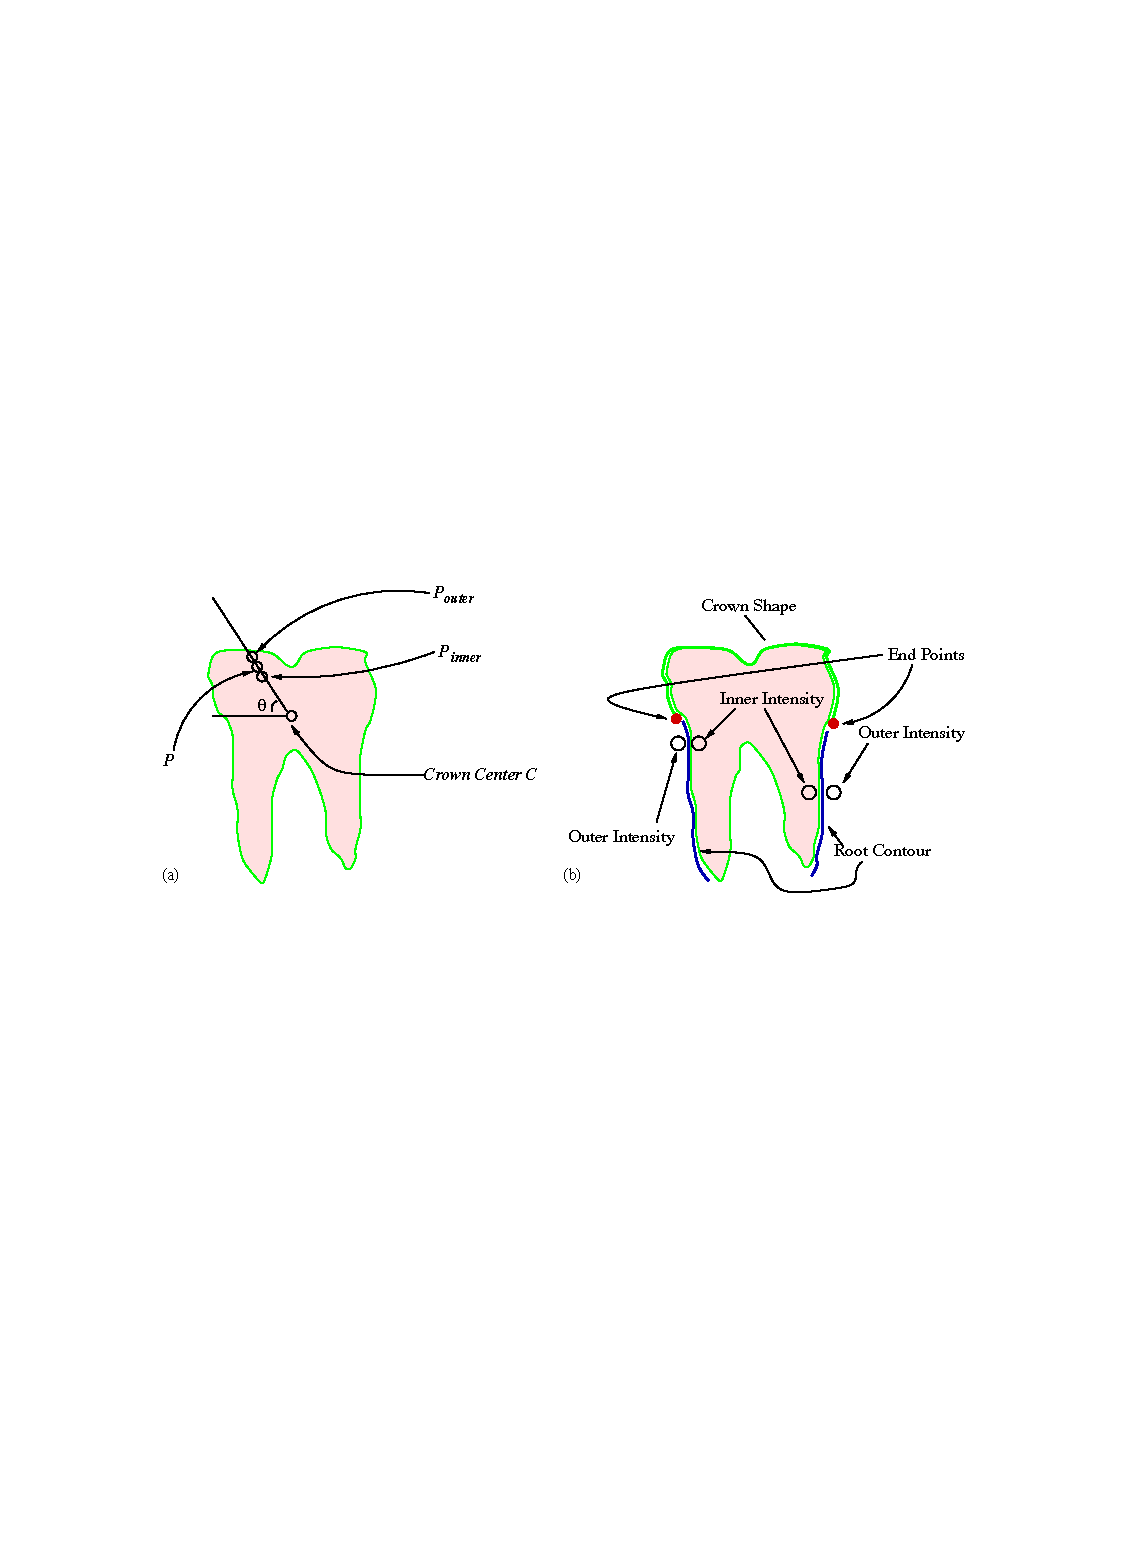
\includegraphics[width=.8\linewidth]{resources/contour-tracing.pdf}
  \caption{Detectie van kroon en wortel (overgenomen uit \cite{jain2004matching}).}
  \label{fig:contour-tracing}
\end{figure}

\subsubsection*{Wortel}

Het eerste en laatste punt uit de contour van de kroon vormen de beginpunten van twee deel-contouren die de wortel afbakenen. Er wordt hier een andere methode gebruikt dan bij de kroon. Aangezien de wortel typisch recht naar beneden beweegt, volgen we nu deze neerwaartse lijn en zoeken in de horizontale nabijheid naar het punt met de meeste kans om op de contour te liggen. Dit wordt nu eenvoudig gedaan door een gemiddelde intensiteit te zoeken links en rechts van een punt net onder het vorige en het contrast verschil te gebruiken als te optimaliseren eigenschap. Figuur \ref{fig:contour-tracing}b toont deze aanpak.

Zo bekomen we uiteindelijk drie stukken van de contour en kunnen we deze samenstellen tot \'e\'en gesloten contour. Het resultaat van zo'n contour bepaling wordt getoond in figuur \ref{fig:contours-01} voor het eerste beeld uit de opgave. Appendix \ref{appendix:contours} geeft een overzicht van alle resultaten.

\subsection*{Nabewerking}

De bekomen contouren bevatten veel fouten in de vorm van losse contour-pixels die te ver naar binnen of buiten liggen. Ook zijn ze zeer onregelmatig en bevatten daarom veel onnuttige details. Voor we deze contouren kunnen vergelijken met de aangeleverde resultaten, moeten we een nabewerking toepassen om er een redelijk masker van te maken.

\begin{figure}
\centering
\begin{subfigure}{.49\textwidth}
  \centering
  \includegraphics[width=.8\linewidth]{../01_crp_enh_contours.tif}
  \caption{Gedetecteerde contouren van \ttt{01.tif}}
  \label{fig:contours-01}
\end{subfigure}
\begin{subfigure}{.49\textwidth}
  \centering
  \includegraphics[width=.8\linewidth]{../01_crp_enh_masks.tif}
  \caption{Zachtere contouren van \ttt{01.tif}}
  \label{fig:masks-01}
\end{subfigure}
\caption{Resultaten van de contour-detectie.}
\label{fig:results-01}
\end{figure}

Dit gebeurt in de \ttt{mask.py} module. Hier wordt de gedetecteerde contour genomen en door middel van verschillende filterende operaties bewerkt tot een \emph{zachtere} versie die meer geschikt is als \emph{masker}. 

Eerst wordt de contour, zoals hij gedetecteerd is, getekend als een vol wit vlak. Vervolgens wordt hierop een \emph{dilatatie} uitgevoerd, waardoor een ruimere figuur beschreven wordt. Deze wordt opnieuw gereduceerd door uitvoeren van een \emph{erodering}. Tot slot wordt het bekomen beeld verzacht met een \emph{vervagende} filter.

Voor de dilatatie werd een kruisvormige structuur gebruikt van 17 bij 17 pixels; voor de erodering eveneens een kruisvormige structuur maar dan van 13 bij 13. Voor de vervagende filter werd een gewone \emph{blur} functie gebruikt me een kernel van 9 bij 9.

In het bekomen beeld werd opnieuw een contour gezocht. Deze is een zachtere versie van de gedetecteerde contour, zonder dat echt veel details verloren gaan. Figuur \ref{fig:masks-01} toont het resultaat  naast de gedetecteerde contouren.

Een laatste stap die ge\"implementeerd werd is een vergelijking met de aangeleverde resultaten. \ttt{compare\_masks.py} maakt een vergelijkende maskering van de bekomen resultaten en de correcte oplossing. Hierbij worden pixels die overeenkomen in beide maskers groen weergegeven, pixels die verkeerd zijn in het rood en pixels die niet gevonden werden in het blauw. Figuur \ref{fig:comparison-01} toont deze resultaten voor het eerste beeld.

Uit deze figuur blijkt dat de resultaten vrij positief zijn. De bovenste snijtanden vertonen een hoofdzakelijk groene kleur, maar mogelijk zijn veel typerende details verloren gegaan. Bij de onderste tanden merken we op dat in het algemeen de wortels niet diep genoeg gedetecteerd zijn. In het geval van de linkse onderste snijtand zien we, doordat de rechtse wortel-contour nagenoeg niet gedetecteerd werd, dat door de manier waarop de contouren gecombineerd worden, er een groot stuk verloren kan gaan in combinatie met de detectie van een verkeerde andere zone.

Appendix \ref{appendix:comparison} toont alle vergelijkende maskers voor de eerste twintig beelden. Hieruit blijft al snel dat de resultaten zeer variabel zijn.

\begin{figure}
  \centering
  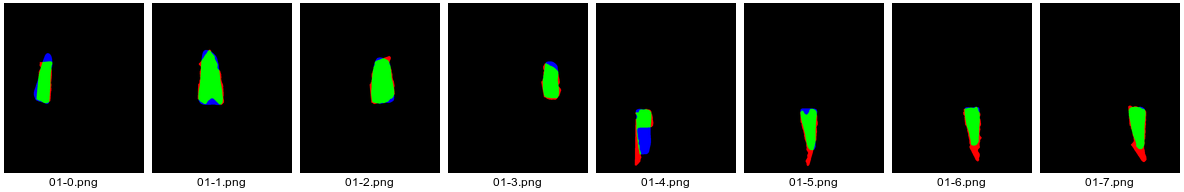
\includegraphics[width=\linewidth]{resources/comparison-01.png}
  \caption{Vergelijking van gedetecteerde maskers met aangeleverde resultaten voor \ttt{01.tif}.}
  \label{fig:comparison-01}
\end{figure}

\subsection*{Parameters}

Tijdens de implementatie werden verschillende \emph{globale} parameters ge\"identificeerd\footnote{De Makefile bevat deze parameters en zorgt er voor dat ze op de juiste manier aangeboden worden aan de verschillende scripts.}:

\begin{description}
\item[crop width]  geeft de breedte aan van het centraal uit te knippen deel van het originele beeld.\\ Waarde: 700 pixels.
\item[crop height] geeft de hoogte aan van het centraal uit te knippen deel van het originele beeld.\\ Waarde: 1100 pixels.
\item[crop top offset] is het deel dat extra verwijderd wordt van de bovenzijde van het uitgeknipte deel. \\ Waarde: 250 pixels.
\item[alpha] is de manueel vastgestelde waarde voor de $\alpha$ parameter bij contrast-stretching. \\ Waarde: 20.
\item[slices] is het aantal splitsingen dat gezocht wordt. Dit is \'e\'en meer dan het aantal tanden. \\ Waarde: 5.
\item[expected jaw split] is de verwachte hoogte van de splitsing tussen de kaken. \\ Waarde: 70\%.
\item[sigma] bepaalt hoe de Gausiaanse waarschijnlijkheidsfunctie voor het bepalen van de splitsing tussen onder- en bovenkaak, rekening houdt met de verwachte locatie.\\ Waarde: 0.4.
\item[inversion top] bepaalt de hoogte van de waarschijnlijkheidsfunctie t.o.v.\ welke ze afgetrokken wordt om een sterk verkleinende waarden te bekomen in de verwachte zone. \\ Waarde: 1.1.
\item[upper length] is de verwachte lengte in pixels van de bovenste tanden.\\ Waarde: 350 pixels.
\item[lower length] is de verwachte length in pixels van de onderste tanden. \\ Waarde" 300 pixels.
\end{description}

Elk van deze parameters is typisch onderhevig aan de doelstellingen en mogelijkheden. Ze kunnen op basis van een \emph{vluchtige} blik op alle beelden bepaald worden zonder specifiek enige beeld te bevoordelen. De belangrijkste uitzonderingen op deze regel zijn \emph{alpha}, \emph{sigma} en \emph{inversion top}. De laatste twee zijn vrij technische parameters die geen uitgesproken invloed hebben op de resultaten. De parameter voor de \emph{contrast stretching} daarentegen wel.

\subsection*{ui.py}

\begin{wrapfigure}{r}{0.49\textwidth}
  \vspace{-1cm}
  \centering
  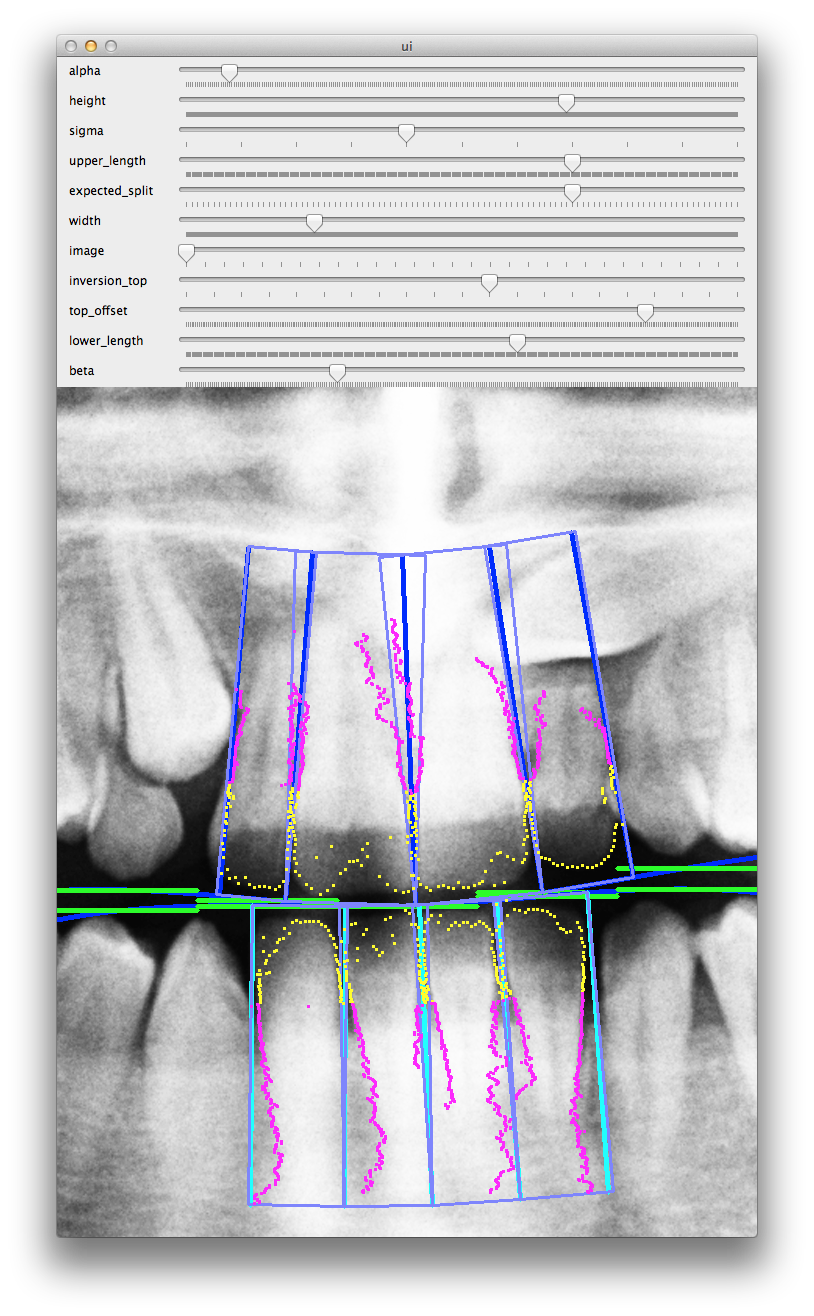
\includegraphics[width=\linewidth]{resources/ui.png}
  \caption{Gebruikers-interface voor het experimenteren met parameters.}
  \label{fig:ui}
  \vspace{-1cm}
\end{wrapfigure}

Dit laatste aspect werd duidelijk toen een bijkomende implementatie van de verschillende modules werd gerealiseerd in de vorm van een overkoepelende gebruikers-interface (\ttt{ui.py}). Deze interface laat toe om alle parameters te wijzigen, terwijl de resultaten onmiddellijk worden weergegeven voor een geselecteerd beeld. Dit laat toe om stapsgewijs te experimenteren met de verschillende parameters. Figuur \ref{fig:ui} toont de interface.

Zo werd op het einde van de implementatie de oorspronkelijk bepaalde waarde voor \emph{alpha}, verder bijgesteld waardoor er sterk verbeterde eind resultaten konden opgetekend worden voor een selectie van de beelden.

\section*{Resultaten en conclusies}

Appendix \ref{appendix:comparison} toont de effectieve resultaten. Buiten enkele uitzonderlijke beelden, is het resultaat overwegend tegenvallend. Zoals vermeld in \cite{jain2004matching} blijkt deze aanpak inderdaad niet voordelig in een volledig geautomatiseerde opstelling. Het aantal parameters en de gevoeligheid van deze parameters toont aan dat het inderdaad eerder een sterk gesuperviseerde methode is.

In bijna elke fase werd uitgegaan van een door een externe bron aangeleverde basis aan informatie: bv.\ voor de splitsing tussen de onder- en bovenkaak; ook bij het splitsen van de individuele tanden zou een helpende hand veel problemen kunnen vermijden, enz.

Het gebruik van de interface om de waarde van \emph{alpha} te verfijnen, toonde \'e\'en van de belangrijkste conclusies aan uit dit project: de kwaliteit van het beeldmateriaal is van zeer groot belang voor deze algoritmes. Indien de contrasten niet op een zorgvuldige manier gecorrigeerd worden, zullen dit soort doelgerichte algoritmes zeer makkelijke falen.

Doorheen de overzichten is een duidelijke trend te merken: die beelden die op het einde een redelijk resultaat laten optekenen t.o.v.\ de aangeleverde voorbeelden, vertonen deze kwaliteit in elke fase van het algoritme. De doelgerichtheid van de verschillende stappen brengt een groeiend positief of negatief resultaat met zich mee.

\'E\'en van de persoonlijke doelstellingen van dit project was om deze redelijk afwijkende methode - t.o.v.\ deze gezien tijdens de cursus - te evalueren. Zonder bijkomende implementaties is het niet met zekerheid vast te stellen, maar vermoedelijk zullen andere methoden op basis van algemene filters, gradi\"enten en \emph{rand detectoren} meer betrouwbare resultaten kunnen opleveren. De auteurs zoeken zelf hun heil in deze richting zoals beschreven in \cite{chen2004tooth}.

Desondanks de tegenvallende resultaten was de implementatie een uitdaging en kwamen veel interessante technieken aan bod: het analyseren van histogrammen om \emph{features} te vinden, het toepassen van eenvoudige geometrische algoritmes om transformaties uit te voeren op delen van het hele beeld, het werken met contouren, enz. Daarnaast was ook het automatiseren van alle stappen op een gestructureerde manier een interessante leerschool. Ofschoon Python, NumPy, SciPy en OpenCV nog veel geheimen hebben, zijn ze een nuttige aanwinst in de persoonlijke gereedschapskoffer.

Maar de tegenvallende resultaten mogen niet volledig toegeschreven worden aan de gevolgde methodologie. Wanneer we bv.\ kijken naar de histogrammen van de kronen in appendix \ref{appendix:crown_histograms}, merken we op dat het eenvoudige algoritme om de eerste Gausiaanse component te vinden verre van perfect is. Nog veel fundamenteler is misschien de slechte keuze die gemaakt werd in de vorm van \emph{contrast stretching}. Ongetwijfeld zorgt een betere voorbereiding van het beeld er voor dat de resultaten drastisch verbeteren.

\subsection*{Tijdsbesteding}

De literatuurstudie, implementatie en het schrijven van het verslag namen samen ongeveer 95 uren in beslag. Een groot deel hiervan was toe te wijzen aan het verkennen van de mogelijkheden van Python, NumPy, SciPy en OpenCV. \'E\'en van de belangrijkste oorzaken van tijdverlies was type-problemen. Dikwijls moesten Numpy lijsten van type veranderd worden voor ze correct konden verwerkt worden. Dit leidde soms tot zoektochten naar alternatieven, om uiteindelijk soms op een minuscule type-verandering uit te komen als zeer eenvoudige oplossing.

Ook de grote overlappen in mogelijkheden tussen de verschillende bibliotheken zorgde voor keuzes waarvan de gevolgen op voorhand soms niet in te schatten waren, met herwerkingen tot gevolg.


\bibliographystyle{alpha}
\bibliography{references}

\newpage

\appendix

\section*{Voorbereidende stappen}

\subsection*{Voorbereide originele beelden}
\label{appendix:prepared-originals}

\begin{figure}[H]
\centering
\includegraphics[width=.9\linewidth]{../enhanced.png}
\caption{Voorbereide originele beelden.}
\label{fig:prepared-originals}
\end{figure}

\subsection*{Originele histogrammen}
\label{appendix:cropped-histograms}

\begin{figure}[H]
\centering
\includegraphics[width=\linewidth]{../cropped_hists.png}
\caption{Originele histogrammen}
\label{fig:cropped-histograms}
\end{figure}

\subsection*{Sigmoids}
\label{appendix:sigmoids}

\begin{figure}[H]
\centering
\includegraphics[width=\linewidth]{../sigmoids.png}
\caption{Sigmoids}
\label{fig:sigmoids}
\end{figure}

\subsection*{Histogrammen na contrast stretching}
\label{appendix:enhanced-histograms}

\begin{figure}[H]
\centering
\includegraphics[width=\linewidth]{../enhanced_hists.png}
\caption{Histogrammen na contrast stretching}
\label{fig:enhanced-histograms}
\end{figure}

\section*{Boven- en onder kaak-splitsing}
\label{appendix:jaw-splits}

\subsection*{Splitsingen}

\begin{figure}[H]
\centering
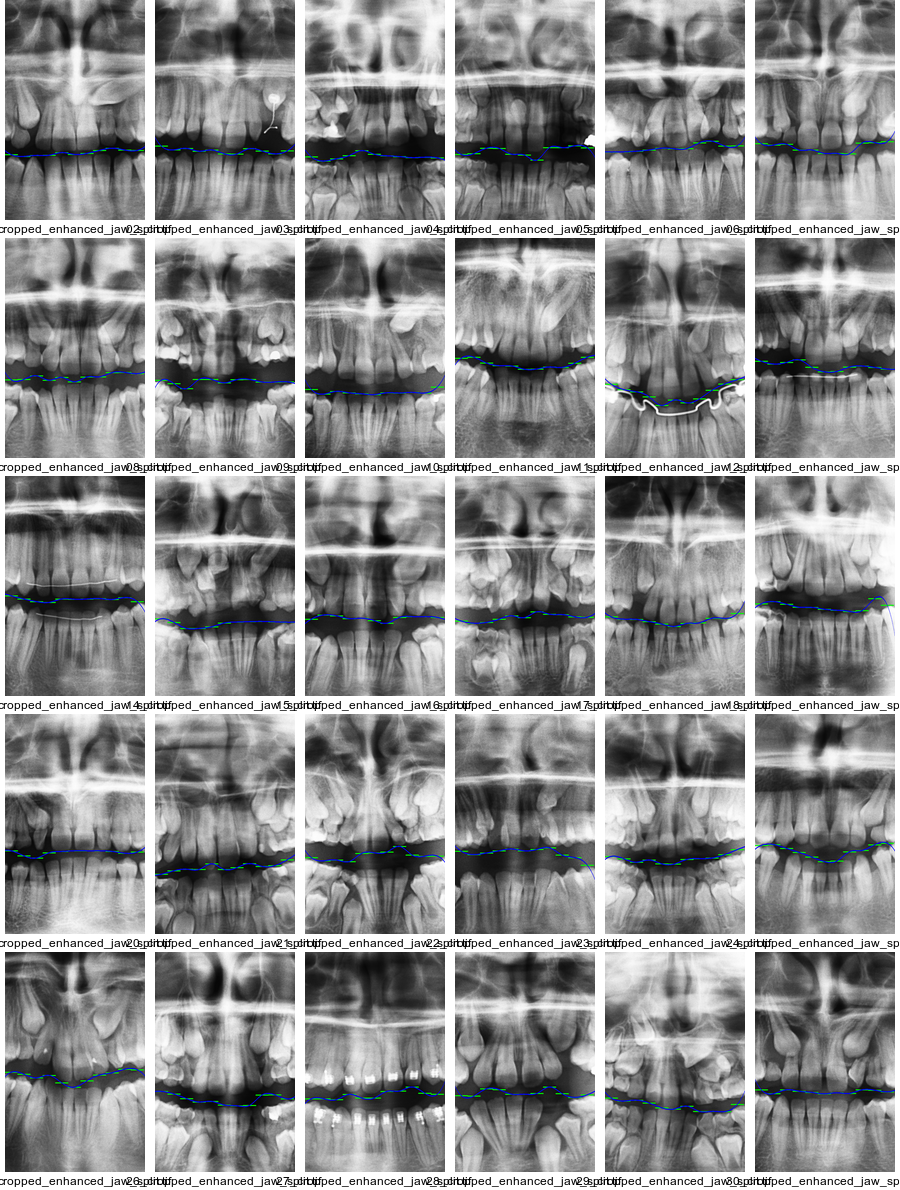
\includegraphics[width=.9\linewidth]{../jaw_splits.png}
\caption{Splitsing van onder- en bovenkaak.}
\label{fig:jaw-splits}
\end{figure}

\subsection*{Histogrammen}

\begin{figure}[H]
\centering
\includegraphics[width=\linewidth]{../jaw_splits_hists.png}
\caption{Histogrammen van onder- en bovenkaak.}
\label{fig:jaw-splits-hists}
\end{figure}


\section*{Individuele snijtand segmentatie}
\label{appendix:teeth-segmentation}

\subsection*{Splitsingen}
\label{appendix:teeth-isolation}

\begin{figure}[H]
\centering
\includegraphics[width=.9\linewidth]{../teeth_iso.png}
\caption{Splitsing van individuele snijtanden.}
\label{fig:teeth-isolation}
\end{figure}

\subsection*{Histogrammen}
\label{appendix:teeth-isolation-hists}

\begin{figure}[H]
\centering
\includegraphics[width=\linewidth]{../teeth_iso_hists.png}
\caption{Histogrammen en aanduiding van individuele snijtanden.}
\label{fig:teeth-isolation-hists}
\end{figure}

\subsection*{ROI's}
\label{appendix:rois}

\begin{figure}[H]
\centering
\includegraphics[width=.9\linewidth]{../roi.png}
\caption{ROI's}
\label{fig:rois}
\end{figure}

\section*{Resulterende contouren en maskers}
\label{appendix:contours}

\subsection*{Gedetecteerde contouren}

\begin{figure}[H]
\centering
\includegraphics[width=.9\linewidth]{../contours.png}
\caption{Contourss}
\label{fig:contours}
\end{figure}

\subsection*{Kroon Histogrammen}
\label{appendix:crown_histograms}

\begin{figure}[H]
\centering
\includegraphics[width=.9\linewidth]{../crown_histograms-0.png}
\caption{Sets 01 tot 10}
\label{fig:crown_histograms-0}
\end{figure}

\begin{figure}[H]
\centering
\includegraphics[width=.9\linewidth]{../crown_histograms-1.png}
\caption{Sets 11 tot 20}
\label{fig:crown_histograms-1}
\end{figure}


\subsection*{Zachte contouren}

\begin{figure}[H]
\centering
\includegraphics[width=.9\linewidth]{../masks.png}
\caption{Maskers}
\label{fig:masks}
\end{figure}

\subsection*{Vergelijking met verwachte resultaat}
\label{appendix:comparison}

\begin{figure}[H]
\centering
\includegraphics[width=.9\linewidth]{../comparison-0.png}
\caption{Vergelijking sets 01 tot 10}
\label{fig:comparison-0}
\end{figure}

\begin{figure}[H]
\centering
\includegraphics[width=.9\linewidth]{../comparison-1.png}
\caption{Vergelijking sets 11 tot 20}
\label{fig:comparison-1}
\end{figure}


\end{document}
